\documentclass{article}
\usepackage[utf8]{inputenc}
\usepackage{geometry}
 \geometry{
 a4paper,
 total={170mm,257mm},
 left=20mm,
 top=20mm,
 }
\usepackage{graphicx}
\usepackage{titling}
\usepackage{enumitem}
\usepackage{float}
\usepackage{caption}
\usepackage{subcaption}
\usepackage{amsmath}
\usepackage{booktabs} % For professional table formatting
\usepackage{appendix}
\usepackage{multirow}
\usepackage{pdfpages} % Package to include PDF pages

\usepackage{hyperref}
\hypersetup{
    colorlinks=true,
    linkcolor=blue,
    filecolor=magenta,      
    urlcolor=cyan,
    pdftitle={Discretization Methods},
    pdfpagemode=FullScreen,
    }

\urlstyle{same}


\title{Exercise Sheet 3}
\author{Dennys Huber}
\date{\today}
 
 \usepackage{fancyhdr}
\fancypagestyle{plain}{%  the preset of fancyhdr 
    \fancyhf{} % clear all header and footer fields
    \fancyfoot[C]{\thepage}
    % \fancyfoot[L]{\thedate}
    \fancyhead[L]{Discretization Methods}
    \fancyhead[R]{\theauthor}
}
\pagestyle{plain}% Set page style to plain.
\makeatletter
\def\@maketitle{%
  \newpage
  \null
  \vskip 1em%
  \begin{center}%
  \let \footnote \thanks
    {\LARGE \@title \par}%
    \vskip 1em%
    {\large \@author}%
    \vskip 1em%
    {\large \@date}%
  \end{center}%
  \par
  \vskip 1em}
\makeatother


\begin{document}

\maketitle

\section{Fourier-Galerking Approximation: Exercise 1}
\subsection{Derivation}
We are considering the variable coefficient problem
\begin{equation}
	\frac{\partial u}{\partial t}+\sin (x) \frac{\partial u}{\partial x}=0
	\label{eq:pde}
\end{equation}
with periodic boundary condition.\\
We assume that $u(x,t)$ is periodic in $x \in [0, 2\pi]$ and use a truncated Fourier series to define
\begin{equation}
	u_N = \sum_{n=0}^N \hat{u}_n(t) \phi_n(x) = \sum_{n=-\frac{N}{2}}^{\frac{N}{2}} \hat{u}_n(t) e^{inx}
	\label{eq:un}
\end{equation}
where the continues expansion coefficients $\hat{u}_n$ are defined as (see Lecture 8)
\begin{equation}
	\hat{u}_n(t) = \frac{1}{2 \pi} \int_0^{2\pi} u(x, t) e^{-inx} dx .
	\label{eq:un_hat}
\end{equation}
We can now substitute $u_N$ into the PDE \eqref{eq:pde}:
\begin{equation}
	\frac{\partial u_N}{\partial t}+\sin (x) \frac{\partial u_N}{\partial x}=0
	\label{eq:un_pde}
\end{equation}
Computing each term
\begin{itemize}
	\item \textit{Time derivative}:
	      \begin{equation}
		      \frac{\partial u_N}{\partial t} = \sum_{n=-\frac{N}{2}}^{\frac{N}{2}} \frac{d \hat{u}_n}{dt} e^{inx}
		      \label{eq:time_der}
	      \end{equation}
	\item \textit{Spatial derivative}:
	      \begin{equation}
		      \frac{\partial u_N}{ \partial x} = \sin (x) \sum_{n=-\frac{N}{2}}^{\frac{N}{2}} \hat{u}_n \frac{d}{dx}\left [ e^{inx} \right] =  \sum_{n=-\frac{N}{2}}^{\frac{N}{2}} i n \hat{u}_n \sin(x)  e^{inx}
		      \label{eq:spat_der}
	      \end{equation}
\end{itemize}
The Residual is now given as follows
\begin{equation}
	R_N(x, t)=\frac{\partial u_N}{\partial t}-\mathcal{L} u_N = \frac{\partial u_N}{\partial t}+\sin (x) \frac{\partial u_N}{\partial x}
\end{equation}
We enforce $\left(R_N, \psi_m\right)_w=0, \forall m \in[-N / 2, N / 2]$, where $\psi_m=\frac{1}{\gamma_m} \phi_m$, so that $\left(\phi_m, \psi_n\right)_w=\delta_{m n}$.
\begin{equation}
	\left(R_N, \psi_m\right)_w = \int_0^{2\pi} \left(\frac{\partial u_N}{\partial t}-\mathcal{L} u_N \right)\overline{\psi_m}wdx = \int_0^{2\pi} \left (  \frac{\partial u_N}{\partial t}+\sin (x) \frac{\partial u_N}{\partial x} \right) \frac{1}{2\pi}e^{-imx} = 0
	\label{eq:res}
\end{equation}
Choosing $w(x) = 1$, and using orthonormal basis $\psi_m(x) = \frac{1}{2\pi}e^{imx}$, we have:
\begin{equation}
	(\phi_n, \psi_m)_w = \int_0^{2\pi} e^{inx} \cdot \frac{1}{2\pi} e^{-imx} dx = \delta_{nm}.
	\label{eq:weight_f}
\end{equation}
We now plugin the results of \eqref{eq:time_der} and \eqref{eq:spat_der} into \eqref{eq:res} we get
\begin{equation}
	\begin{aligned}
		\left(R_N, \psi_m\right)_w &= \int_0^{2\pi} \left( \sum_{n=-\frac{N}{2}}^{\frac{N}{2}} \frac{d \hat{u}_n}{dt} e^{inx} + \sin(x) \sum_{n=-\frac{N}{2}}^{\frac{N}{2}} i n \hat{u}_n e^{inx} \right) \cdot \frac{1}{2\pi} e^{-imx} dx.
	\end{aligned}
	\label{eq:res_der}
\end{equation}
First lets simplify the first term inside the integral
\begin{equation}
	\int_0^{2 \pi} \sum_{n=-\frac{N}{2}}^{\frac{N}{2}}  \frac{d \hat{u}_n}{dt} e^{inx} \frac{1}{2\pi} e^{-imx} dx = \frac{1}{2\pi}\sum_{n=-\frac{N}{2}}^{\frac{N}{2}}  \frac{d \hat{u}_n}{dt} \int_0^{2 \pi} e^{i(n-m)x} = \frac{1}{2\pi}\sum_{n=-\frac{N}{2}}^{\frac{N}{2}}  \frac{d \hat{u}_n}{dt} 2 \pi \delta_{nm} = \frac{d \hat{u}_m}{dt}
	\label{eq:res_first}
\end{equation}
For the second term we can rewrite sine as
\begin{equation}
	\sin(x) = \frac{e^{ix} - e^{-ix}}{2i}
	\label{eq:sin_exp}
\end{equation}
and then substitute it into the second term
\begin{equation}
	\begin{aligned}
		\int_0^{2\pi} \sum_{n=-\frac{N}{2}}^{\frac{N}{2}} i n \hat{u}_n \sin(x)  e^{inx} \frac{1}{2\pi} e^{-imx} dx & = \frac{1}{2\pi}  \sum_{n=-\frac{N}{2}}^{\frac{N}{2}} i n \hat{u}_n  \int_0^{2\pi} \frac{e^{ix} - e^{-ix}}{2i} e^{i(n-m)x} dx       \\
		                                                                                             & =  \frac{1}{2\pi}  \sum_{n=-\frac{N}{2}}^{\frac{N}{2}} i n \hat{u}_n  \int_0^{2\pi} \frac{e^{i(n-m + 1)x} - e^{i(n-m -1) x}}{2i} dx \\
		\label{eq:res_second}
	\end{aligned}
\end{equation}
using the orthogonality property again, this integral becomes non-zero only when:
\begin{equation}
	\begin{aligned}
		n - m + 1 & = 0 \Rightarrow n = m -1   \\
		n - m - 1 & = 0 \Rightarrow n = m  + 1
	\end{aligned}
	\label{eq:res_second_non_zero}
\end{equation}
Therefore the second term becomes
\begin{equation}
	i(m-1)\hat{u}_{m-1} \frac{1}{2\pi} \frac{\int_0^{2\pi} e^0 dx}{2i} - i(m+1) \hat{u}_{m+1} \frac{1}{2\pi} \frac{\int_0^{2\pi} e^0 dx}{2i} = \frac{1}{2}  \left [ (m - 1)\hat{u}_{m-1} - (m+1) \hat{u}_{m+1}  \right]
	\label{eq:res_second_final}
\end{equation}
Now we can combine both terms, resulting in
\begin{equation}
	\frac{d \hat{u}_m}{dt} + \frac{1}{2} \left [ (m - 1)\hat{u}_{m-1} - (m+1) \hat{u}_{m+1}  \right] = 0
	\label{eq:res_eqs}
\end{equation}
Rearranging this result leads to our systems of ODEs for the Fourier-Galerking approximation
\begin{equation}
	\frac{d \hat{u}_m}{dt} = \frac{ (m + 1)\hat{u}_{m+1} - (m-1) \hat{u}_{m-1}}{2}
	\label{eq:FG_ODEs}
\end{equation}
and the initial condition is given as 
\begin{equation}
	\hat{u}_m (0) = \frac{1}{2\pi} \int_0^{2\pi}g(x)e^{-imx}dx
	\label{eq:init}
\end{equation}
\subsection{Is $P_N u = u_N?}
If we apply the Fourier-Galerking Approximation to the equation satisfied by the exact solution $u$, we get
\begin{equation}
	\frac{d \hat{u}_m}{dt} = \frac{ (m + 1)\hat{u}_{m+1} - (m-1) \hat{u}_{m-1}}{2} + \epsilon_T
	\label{eq:trunc_err}
\end{equation}
where $\epsilon_T$ is the truncation error. In order for the $P_N u = u_N$ to hold $\epsilon_T$ has to be $0$.
\begin{equation}
	P_N\left(\frac{\partial u}{\partial t} + \sin(x)\frac{\partial u}{\partial x}\right) = \frac{\partial P_N u}{\partial t} + P_N\left(\sin(x)\frac{\partial u}{\partial x}\right) = P_N(0) = 0
	\label{eq:}
\end{equation}
The Problem is that in general
\begin{equation}
	P_N\left(\sin(x)\frac{\partial u}{\partial x}\right) \neq \sin(x) \frac{\partial P_N u}{\partial x}
	\label{eq:prob}
\end{equation}
because when we are multiplying $\sin(x) = \frac{e^{ix} - e^{-ix}}{2i}$ with $\frac{\partial u}{dx} = \sum_{-\infty}^{\infty} i n \hat{u}_n e^{inx}$ it creates frequencies that are outside our truncated space, created by the projection into finite space by $P_N$.


\section*{Exercise 2}
\subsection*{Wave Speed}
We assume that the solution to the finite difference scheme is rightward traveling wave
\begin{equation}
	v(x,t) = e^{ik(x-c_6t)}
	\label{eq:wave_sol}
\end{equation}
We plug \eqref{eq:wave_sol} into our finite difference scheme \eqref{eq:final}
\begin{equation}
	\begin{aligned}
		-ikc_6 e^{ik(x_j-c_6t)} & = -\frac{c}{60 \Delta x} [-e^{ik(x_{j-3}-c_6t)} + 9e^{ik(x_{j-2}-c_6t)} -45 e^{ik(x_{j-1}-c_6t)} \\
		                        & + 45e^{ik(x_{j+1}-c_6t)}-9e^{ik(x_{j+2}-c_6t)} + e^{ik(x_{j+3}-c_6t)} ]
	\end{aligned}
	\label{eq:wave_scheme}
\end{equation}
Now divided both side by $ e^{ik(x_j-c_6t)}$
\begin{equation}
	\begin{aligned}
		-ikc_6 & = -\frac{c}{60 \Delta x} [-e^{ik(x_{j-3}-x_j)} + 9e^{ik(x_{j-2}-x_j)} -45 e^{ik(x_{j-1}-x_j)}                                                                \\
		       & \quad + 45e^{ik(x_{j+1}-x_j)}-9e^{ik(x_{j+2}-x_j)} + e^{ik(x_{j+3}-x_j)} ]                                                                                   \\
		       & = -\frac{c}{60 \Delta x} \left [-e^{-3ik \Delta x} + 9e^{-2ik\Delta x} -45 e^{-ik \Delta x} + 45e^{ik\Delta x} -9e^{2ik \Delta x} + e^{3ik\Delta x} \right ]
	\end{aligned}
\end{equation}
We can now use the following formula $e^{ik \phi} - e^{-ik \phi} = 2i \sin (k \phi)$ to simplify the equation even further
\begin{equation}
	\begin{aligned}
		-ikc_6 & =  -\frac{c}{60 \Delta x} \left [ 2i \sin (3k \Delta x ) - 18i \sin (2k \Delta x) + 90i \sin (k \Delta x) \right] \\
		       & = -\frac{c}{30 \Delta x}i  \left [ \sin (3k \Delta x) - 9 \sin (2k \Delta x) + 45 \sin (k \Delta x) \right]       \\
	\end{aligned}
	\label{eq:pairs}
\end{equation}
Dividing by $-ik$ we end up with the wave speed for the 6th order approximation
\begin{equation}
	c_6(k) = c\frac{45 \sin (k \Delta x) - 9 \sin (2k \Delta x) + \sin (3k \Delta x) }{30 k\Delta x}
	\label{eq:wave_speed}
\end{equation}
\subsection*{Phase Error}
For the $2m$-order scheme we can define the phase error as
\begin{equation}
	e_m(k)=\left|\frac{u(x, t)-v(x, t)}{u(x, t)}\right|=\left|1-e^{i k\left(c-c_m\right) t}\right| \approx k t\left|c-c_m(k)\right|
	\label{eq:phase_error}
\end{equation}
Now using our result in \eqref{eq:wave_speed} we can define the phase error for a 6th order scheme as follows
\begin{equation}
	e_6(k, t)=kct\left|1- \frac{45 \sin (k \Delta x) - 9 \sin (2k \Delta x) + \sin (3k \Delta x) }{30 k\Delta x}\right|
	\label{eq:6phase_error}
\end{equation}
To measure the accuracy of the 6th scheme, let's introduce the number of grid points per waive length
\begin{equation}
	p = \frac{\lambda}{\Delta x}= \frac{2 \pi}{k \Delta x}
	\label{eq:n_gp}
\end{equation}
and the number of time the solution returns to itself, due to the periodicity
\begin{equation}
	\nu = \frac{ct}{\lambda}
	\label{eq:periodicity}
\end{equation}
Rewriting the phase error \eqref{eq:6phase_error} in terms of $p$ for $k$ and $\nu$ for $t$ results in
\begin{equation}
	\begin{aligned}
		e_6(p, \nu) & = \frac{2 \pi}{(\lambda/ \Delta x) \Delta x} c \frac{\nu \lambda}{c} \left|1- \frac{45 \sin (2 \pi p^{-1}) - 9 \sin (2 \cdot 2 \pi p^{-1}) + \sin (3 \cdot 2 \pi p^{-1}) }{(30 \cdot 2 \pi p^{-1})}\right| \\
		            & = 2 \pi \nu \left|1- \frac{45 \sin (2 \pi p^{-1}) - 9 \sin (4 \pi p^{-1}) + \sin (6 \pi p^{-1})}{(60 \pi p^{-1})}\right|                                                                                   \\
	\end{aligned}
	\label{eq:6phase_error_pnu}
\end{equation}
If we now perform a leading-order approximation ($p \rightarrow \infty$) this means the terms including $p^{-1}$ become small we can use the Taylor series expansion for $\sin$, which is given by the following formula
To perform a leading-order approximation as $p \to \infty$, we use the Taylor series expansion for sine:
\begin{equation}
	\sin(x) = \sum_{n=0}^{\infty} \frac{(-1)^n}{(2n + 1)!}x^{2n+1} = x - \frac{x^3}{3!} + \frac{x^5}{5!} - \frac{x^7}{7!} + \ldots \tag{30}
\end{equation}
e now expand each sine term in the numerator:
For $\sin(2\pi p^{-1})$:
\begin{equation}
	\sin(2\pi p^{-1}) = 2\pi p^{-1} - \frac{(2\pi p^{-1})^3}{3!} + \frac{(2\pi p^{-1})^5}{5!} - \frac{(2\pi p^{-1})^7}{7!} + \mathcal{O}(p^{-9})
\end{equation}
For $\sin(4\pi p^{-1})$:
\begin{equation}
	\sin(4\pi p^{-1}) = 4\pi p^{-1} - \frac{(4\pi p^{-1})^3}{3!} + \frac{(4\pi p^{-1})^5}{5!} - \frac{(4\pi p^{-1})^7}{7!} + \mathcal{O}(p^{-9})
\end{equation}
For $\sin(6\pi p^{-1})$:
\begin{equation}
	\sin(6\pi p^{-1}) = 6\pi p^{-1} - \frac{(6\pi p^{-1})^3}{3!} + \frac{(6\pi p^{-1})^5}{5!} - \frac{(6\pi p^{-1})^7}{7!} + \mathcal{O}(p^{-9})
\end{equation}
Now we calcualte the numerator for each term of each order.\newline
For the first order terms:
\begin{equation}
	45\left( 2 \pi p^{-1}\right) - 9\left(4 \pi p^{-1}\right) + \left(6 \pi p^{-1}\right) = (90 - 36 + 6) \pi p^{-1} = 60 \pi p^{-1}
\end{equation}
For the third order terms:
\begin{equation}
	45\left( 8 \pi^3 p^{-3}\right) - 9\left(64 \pi^3 p^{-3}\right) + \left(216 \pi^3 p^{-3}\right) = (360 - 576 + 216) \pi^3 p^{-3} = 0 \pi^3 p^{-3} = 0
\end{equation}
For the fifth order terms:
\begin{equation}
	45\left( 32 \pi^5 p^{-5}\right) - 9\left(1024 \pi^5 p^{-5}\right) + \left(7776 \pi^5 p^{-5}\right) = (1440 - 9216 + 7776) \pi^5 p^{-5} = 0 \pi^5 p^{-5} = 0
\end{equation}
and seventh order terms:
\begin{equation}
	\begin{aligned}
		 & 45\left(-\frac{128\pi^7}{5040}p^{-7}\right) - 9\left(-\frac{16384\pi^7}{5040}p^{-7}\right) + \left(-\frac{279936\pi^7}{5040}p^{-7}\right) \\
		 & = -\frac{45 \cdot 128\pi^7}{5040}p^{-7} + \frac{9 \cdot 16384\pi^7}{5040}p^{-7} - \frac{279936\pi^7}{5040}p^{-7}                          \\
		 & = -\frac{5760\pi^7}{5040}p^{-7} + \frac{147456\pi^7}{5040}p^{-7} - \frac{279936\pi^7}{5040}p^{-7}                                         \\
		 & = \frac{-5760 + 147456 - 279936}{5040}\pi^7p^{-7}                                                                                         \\
		 & = \frac{-138240}{5040}\pi^7p^{-7}                                                                                                         \\
		 & = \frac{-192}{7}\pi^7p^{-7}                                                                                                               \\
	\end{aligned}
\end{equation}
Now, substituting back into our original expression:
\begin{equation}
	\begin{aligned}
		e_6(p, \nu) & = 2 \pi \nu \left|1- \frac{60 \pi p^-{1}}{60 \pi p^-{1} } + \frac{\frac{-192}{7}\pi^7p^{-7}}{(60 \pi p^{-1})}\right| \\
		            & = 2\pi\nu \left|\frac{192}{420}\pi^6 p^{-6}\right|                                                                   \\
		            & = 2\pi\nu \left|\frac{16}{35}\pi^6 p^{-6}\right|                                                                     \\
	\end{aligned}
\end{equation}
We can remove the absolute brackets due to p being a large postive number, resulting in the final step:
\begin{equation}
	\begin{aligned}
		e_3(p, \nu) & = 2\pi\nu \frac{16}{35}\pi^6 p^{-6} = \frac{\pi \nu}{70} \left ( \frac{2\pi}{p}\right)^6 \\
	\end{aligned}
\end{equation}
Let's assume we can accept an error $\epsilon_p$ after $\nu$ periods of evolution. 
We can now derive $p_3(\epsilon_p, \nu)$ the number of points per wavelength required to ensure the phase error is bounded by $\epsilon_p$
\begin{equation}
	\begin{aligned}
		e_3(p, \nu)                               & = \frac{\pi \nu}{70} \left ( \frac{2\pi}{p} \right)^6 \\
		\frac{70 e_3(p, \nu)}{\pi \nu}            & =\left ( \frac{2\pi}{p} \right)^6                     \\
		\frac{70 e_3(p, \nu)}{\pi \nu}            & =\left ( \frac{2\pi}{p} \right)^6                     \\
		\sqrt[6]{\frac{70 e_3(p, \nu)}{\pi \nu} } & =  \frac{2\pi}{p}                                     \\
		\sqrt[6]{\frac{70 e_3(p, \nu)}{\pi \nu}}  & = \frac{2\pi}{p}                                      \\
		p                                         & = 2 \pi \sqrt[6]{\frac{\pi \nu}{70e_3(p, \nu)} }
	\end{aligned}
	\label{eq:bound}
\end{equation}
Hence the bound is given as
\begin{equation}
	p_3(\epsilon_p, \nu) \geq 2 \pi \sqrt[6]{\frac{\pi \nu}{70\epsilon_p} }
	\label{eq:bound_final}
\end{equation}
If we now compare the 2nd, 4th, and 6th order schemes using $\epsilon_p = 0.1$ and $\epsilon_p = 0.01$ in Table~\ref{tab:scheme_comparison}, we can observe that for $\epsilon_p = 0.1$, increasing the order doesn't yield much gain, except when integration times are very long (high values of $\nu$). For $\epsilon_p = 0.01$, we observe that higher order schemes become more beneficial even at lower integration times. 
Although the difference between the 2nd order and 4th order schemes is more significant at this error level, if we further decrease the error tolerance and hence increase the required accuracy, the 6th order scheme will become even more beneficial. This trend becomes particularly pronounced for very small error tolerances (e.g., $\epsilon_p = 10^{-5}$).
Our analysis shows that the computational efficiency advantage of higher order schemes increases with stricter accuracy requirements.
In conclusion, the 6th order scheme is recommended when either higher accuracy is required or when simulating over long periods of time that require capturing many oscillations of the solution.

\begin{table}[H]
    \centering
    \begin{tabular}{|c|c|c|c|}
        \hline
        $\epsilon_p$ & 2nd Order Scheme ($p_1$) & 4th Order Scheme ($p_2$) & 6th Order Scheme ($p_3$) \\
        \hline
        0.1 & $p_1 \geq 20\sqrt[2]{\nu}$ & $p_2 \geq 7\sqrt[4]{\nu}$ & $p_3 \geq 5.5\sqrt[6]{\nu}$ \\
		\hline
        0.01 & $p_1 \geq 64\sqrt[2]{\nu}$ & $p_2 \geq 13\sqrt[4]{\nu}$ & $p_3 \geq 8\sqrt[6]{\nu}$ \\
        \hline
    \end{tabular}
    \caption{Comparison of numerical scheme requirements for different error tolerances ($\epsilon_p$)}
    \label{tab:scheme_comparison}
\end{table}


\section{Scalar Hyperbolic Problem}
This exercise is dedicated on solving a scalar hyperbolic problem given as
\begin{equation}
	\begin{gathered}
		\frac{\partial u(x, t)}{\partial t}=-2 \pi \frac{\partial u(x, t)}{\partial x} \\
		u(0, t)=u(2 \pi, t) \\
		u(x, 0)=\exp [\sin (x)]
	\end{gathered}
\end{equation}
where $u(x,t) \in C^\infty[0, 2\pi]$ is assumed periodic. This represents a wave propagating at velocity $2\pi$ in the positive x-direction, while keeping its shape.
This problem is in particular appealing due to the existence of a known analytical solution
\begin{equation}
	u(x, t)=\exp [\sin (x-2 \pi t)],
\end{equation}
making it ideal to benchmark different numerical differentiation methods.
For the time integration, the fourth-order Runga-Kutta method was implemented, which provides high accuracy for temporal discretization.
Thus being able to focus on the analysis of the following three different spatial discretization schemes:
\begin{itemize}
	\item Second-order centered finite difference approximation
	      \begin{equation}
		      \left.\frac{d u}{d x}\right|_{x_j}=\frac{u_{j+1}-u_{j-1}}{2 \Delta x} .
	      \end{equation}
	\item Fourth-order centered finite difference approximation
	      \begin{equation}
		      \left.\frac{d u}{d x}\right|_{x_j}=\frac{u_{j-2}-8 u_{j-1}+8 u_{j+1}-u_{j+2}}{12 \Delta x} .
	      \end{equation}
	\item Global infinite-order approximation using the Odd Fourier method.
	      \begin{equation}
		      \left.\frac{d u}{d x}\right|_{x_j}=\sum_{i=0}^N \tilde{D}_{j i} u_i
	      \end{equation}
\end{itemize}
By looking into the $L_\infty$ error convergence rates and their long-term behaviors, we can evaluate their efficiency, accuracy, and stability characteristics for scalar hyperbolic problems.

\subsection{Convergence Analysis}
The $L_\infty$ error data in Table~\ref{tab:hyperbolic_error} and the corresponding convergence rates in Table~\ref{tab:hyperbolic_rates} for the problem at $t = \pi$ reveals distinct coverngence behaviors.
\begin{itemize}
	\item \textbf{Second-Order Scheme}
	      \begin{itemize}
		      \item Starts with a rather high error and steadily converges as N increases.
		      \item Achieves a final error ($N=2048$) of $1.26 \times 10^{-4}$ .
		      \item The stabilization of the convergence rate happenst at $N \geq 128$ and $\approx 2.0$, perfectly reflecting the theoretical second order accuracy.
	      \end{itemize}
	\item \textbf{Fourth-Order Scheme}
	      \begin{itemize}
		      \item Has an initial error which is lower than the second order scheme.
		      \item Also shows significantly faster error reduction rate.
		      \item Reaching a final error value ($N=2048$) of $1.45 \times 10^{-9}$.
		      \item Convergences rate stabilizes at $\approx 4.0$ for $N \geq 512$, reflecting the theoretical fourth-order accuracy.
	      \end{itemize}
		  \item \textbf{Fourier Scheme}
      \begin{itemize}
              \item Shows dramatically lower errors even at low resolution compared to the other methods.
              \item Achieves extremely rapid initial convergence with a rate of 15.15 between N=8 and N=16.
              \item Reaches machine precision at approximately N=16 with an error of $2.28 \times 10^{-8}$.
              \item After reaching machine precision, error remains constant around $6.3 \times 10^{-9}$ for higher resolutions up to N=512.
              \item Truncation to zero error at N=1024 and N=2048 indicates numerical precision limits.
      \end{itemize}
\end{itemize}
\begin{table}[H]
	\centering
	\begin{tabular}{|c|c|c|c|}
		\hline
		$N$  & Second Order          & Fourth Order          & Fourier                \\
		\hline
		8    & $1.73 \times 10^{0}$  & $6.38 \times 10^{-1}$ & $8.31 \times 10^{-4}$  \\
		16   & $1.06 \times 10^{0}$  & $2.02 \times 10^{-1}$ & $2.28 \times 10^{-8}$  \\
		32   & $4.42 \times 10^{-1}$ & $2.13 \times 10^{-2}$ & $6.20 \times 10^{-9}$  \\
		64   & $1.31 \times 10^{-1}$ & $1.41 \times 10^{-3}$ & $6.34 \times 10^{-9}$  \\
		128  & $3.26 \times 10^{-2}$ & $9.16 \times 10^{-5}$ & $6.36 \times 10^{-9}$  \\
		256  & $8.06 \times 10^{-3}$ & $5.83 \times 10^{-6}$ & $6.36 \times 10^{-9}$  \\
		512  & $2.01 \times 10^{-3}$ & $3.74 \times 10^{-7}$ & $6.36 \times 10^{-9}$  \\
		1024 & $5.03 \times 10^{-4}$ & $2.94 \times 10^{-8}$ & $0.00 \times 10^{0}$   \\
		2048 & $1.26 \times 10^{-4}$ & $7.80 \times 10^{-9}$ & $0.00 \times 10^{0}$   \\
		\hline
	\end{tabular}
	\caption{$L_{\infty}$-Error for the Scalar Hyperbolic Problem at $t = \pi$}
	\label{tab:hyperbolic_error}
\end{table}
\begin{table}[H]
	\centering
	\begin{tabular}{|c|c|c|c|}
		\hline
		$N$  & Second Order & Fourth Order & Fourier \\
		\hline
		16   & 0.71         & 1.66         & 15.15   \\
		32   & 1.26         & 3.24         & 1.88    \\
		64   & 1.75         & 3.92         & -0.03   \\
		128  & 2.01         & 3.95         & -0.00   \\
		256  & 2.01         & 3.97         & 0.00    \\
		512  & 2.00         & 3.96         & -0.00   \\
		1024 & 2.00         & 3.67         & inf     \\
		2048 & 2.00         & 1.91         & nan     \\
		\hline
	\end{tabular}
	\caption{Convergence Rates for the Scalar Hyperbolic Problem}
	\label{tab:hyperbolic_rates}
\end{table}
In conclusion, the observed convergence rates match the theoretical expectation for the finite difference schemes, while the Fourier method demonstrates spectacular convergence characteristics. It shows an extremely rapid initial error reduction (rate of 15.15), quickly reaching machine precision at merely N=16, after which the error remains constant due to floating-point limitations.\\
\\
In order to achieve the same error as the second-order scheme at $N=2048$ ($1.26 \times 10^{-4}$), the fourth-order scheme requires only approximately $N=128$ ($9.16 \times 10^{-5}$) grid points, while the Fourier scheme reaches far better accuracy with just $N=8$ ($8.31 \times 10^{-4}$) and dramatically better at $N=16$ ($2.28 \times 10^{-8}$). This demonstrates the exceptional efficiency of the spectral method, which achieves accuracy orders of magnitude better with far fewer grid points. These results demonstrate that the Fourier method should be the clear choice for problems with smooth, periodic solutions, where it can provide machine-precision accuracy with minimal computational resources.\\
\\
One final important note is how I addressed the challenge of $\pi$ being irrational, which means that any fixed time step $dt$ would likely not divide it evenly, making it difficult to reach $t_{final} = \pi$. I solved this issue, by setting $dt=0.001$ for all methods and then instead of taking $\pi$ as my $t_{final}$, I used:
\begin{equation}
	t^\prime_{final} = dt \cdot \lfloor t_{final} / dt \rfloor
	\label{eq:tfinal}
\end{equation}

\subsection{Longterm Convergence}
In this final exercise we analyze the longtime convergence behavior of the second-order ($N=200$) and spectral Fourier method ($N=10$), when solving the scalar hyperbolic problem, which is depicted in Figure~\ref{fig:figureLabel}. When looking at the time steps $t=0, 100, 200$ we can observe the following:
\begin{itemize}
	\item \textbf{Initial conditions ($t=0$)}
	      \begin{itemize}
		      \item \textbf{Second-Order Method}: This being the initial condition the analytical and numerical solution are identical.
		      \item \textbf{Spectral Fourier Method}: Similar to the second-order method the analytical and numerical are identical.
	      \end{itemize}
	\item \textbf{Medium term ($t=100$)}
	      \begin{itemize}
		      \item \textbf{Second-Order Method}: Beginning to show phase and amplitude errors. The numerical solution has small oscillations are visible near steep gradients, furthermore  the solution is slightly shifted to the right.
		      \item \textbf{Spectral Fourier Method}: Even with just $10$ grid points, the numerical solution maintains the identical shape to the analytical solution.
	      \end{itemize}

	\item \textbf{Long term ($t=200$)}
	      \begin{itemize}
		      \item \textbf{Second-Order Method}: Shows substantial degradation with the numerical solution now being noticeably out of phase. Around $x=5$ we can observe weird oscillations, particular in the region around $x=5$, which indicates numerical instability.
		      \item \textbf{Spectral Fourier Method}: Continues of being identical to the analytical solution.
	      \end{itemize}
\end{itemize}
These results lead to the following four key observations:
\begin{enumerate}
	\item \textbf{Stability}: Second Order method over time starts to accumulate phase errors and develops instabilities, while the spectral Fourier method maintains an exact solution.
	\item \textbf{Efficiency}: The spectral method is significantly more efficient by representing very accurate numerical solution with 20 fold less grid points, compared to the second order.
	\item \textbf{Dispersion}: The second order method showed typical dispersion characteristics, where different components propagate at different speeds, leading to phase errors. The spectral method didn't show any signs of dispersion characteristics.
	\item \textbf{Resolution}: This comparison showed how dramatically better the Fourier method (global) can capture propagation dynamics with fewer grid points.
\end{enumerate}
\begin{figure}[H]
	\centering
	\begin{subfigure}{0.5\textwidth}
		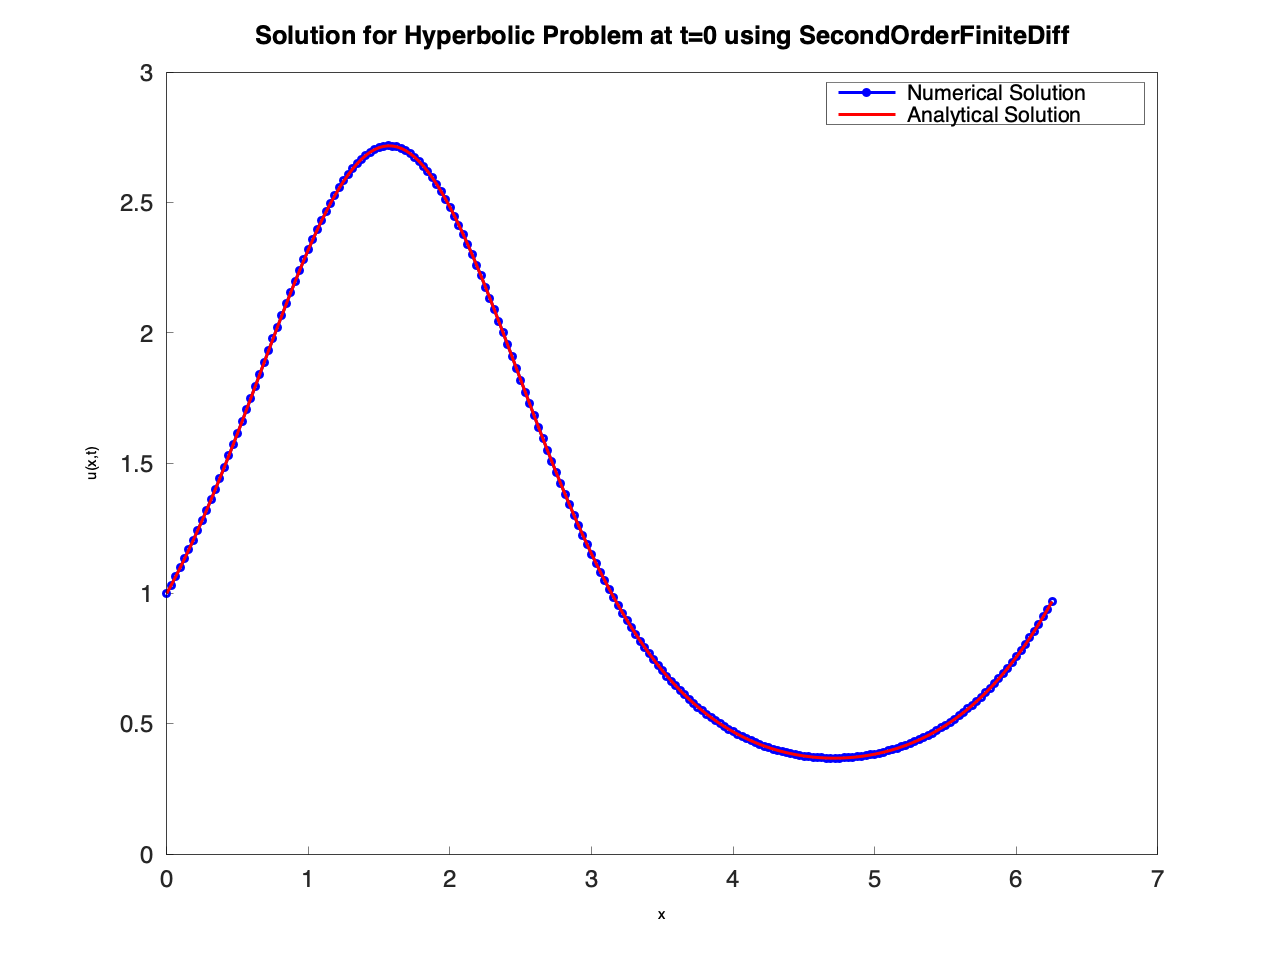
\includegraphics[width=\textwidth]{media/hyperbolic_SecondOrderFiniteDiff_0.png}
		\caption{Second Order at $t=0$}
		\label{sfig:sublabel1}
	\end{subfigure}%
	~
	\begin{subfigure}{0.5\textwidth}
		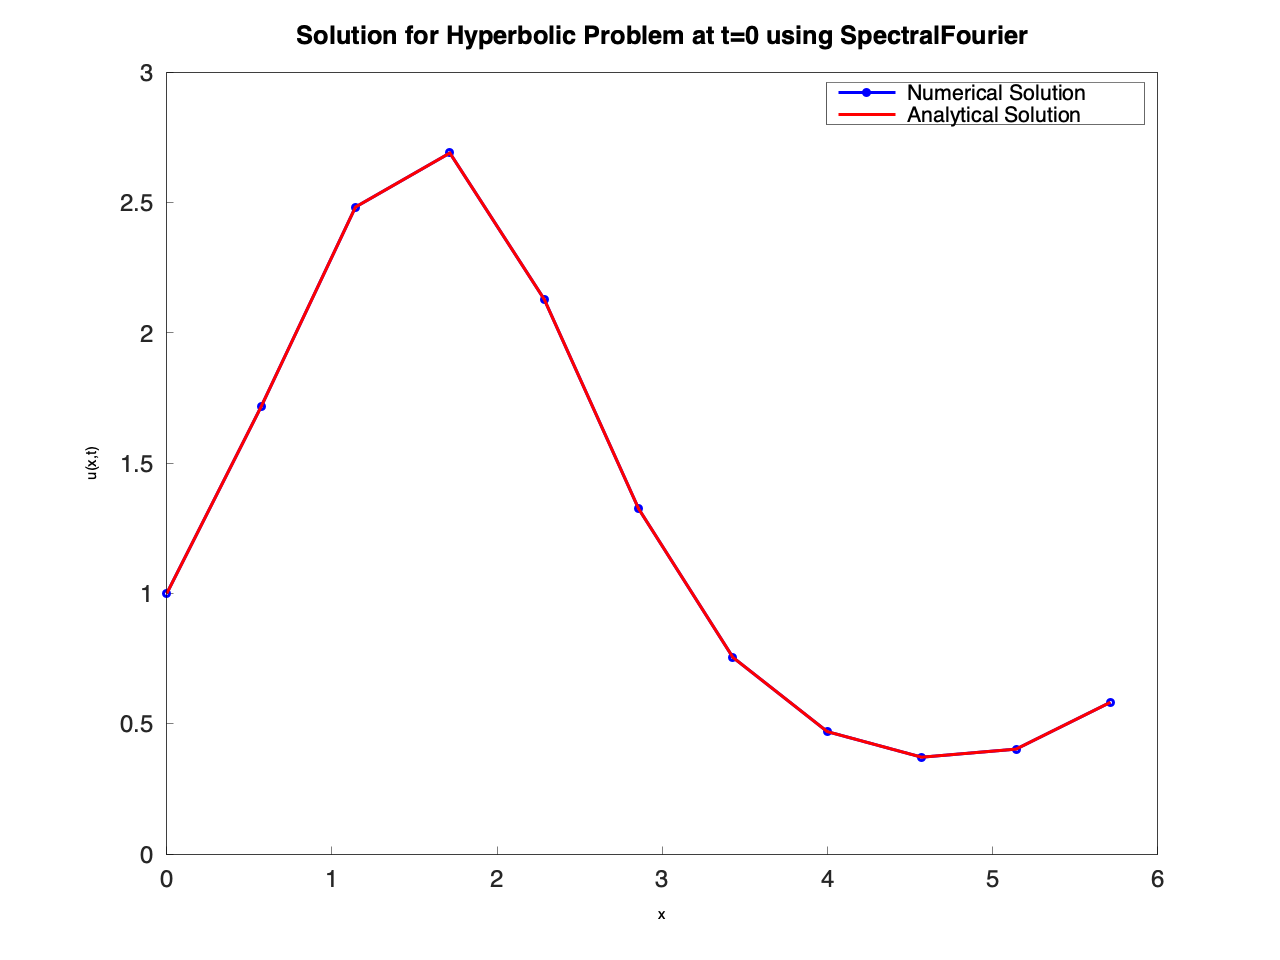
\includegraphics[width=\textwidth]{media/hyperbolic_SpectralFourier_0.png}
		\caption{Spectral Fourier at $t=0$}
		\label{sfig:sublabel2}
	\end{subfigure}\\
	\begin{subfigure}{0.5\textwidth}
		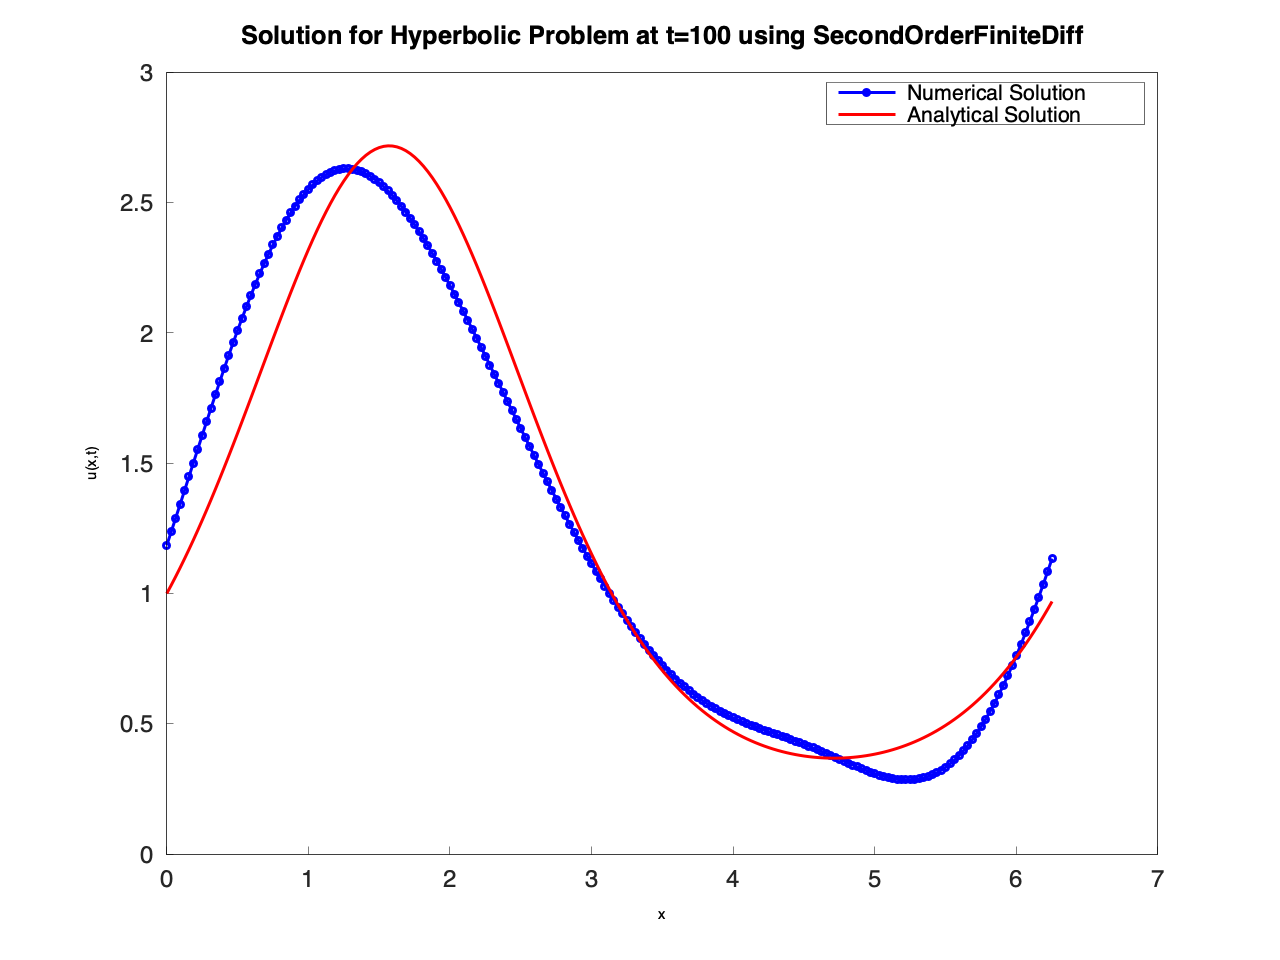
\includegraphics[width=\textwidth]{media/hyperbolic_SecondOrderFiniteDiff_100.png}
		\caption{Second Order at $t=100$}
		\label{sfig:sublabel3}
	\end{subfigure}%
	~
	\begin{subfigure}{0.5\textwidth}
		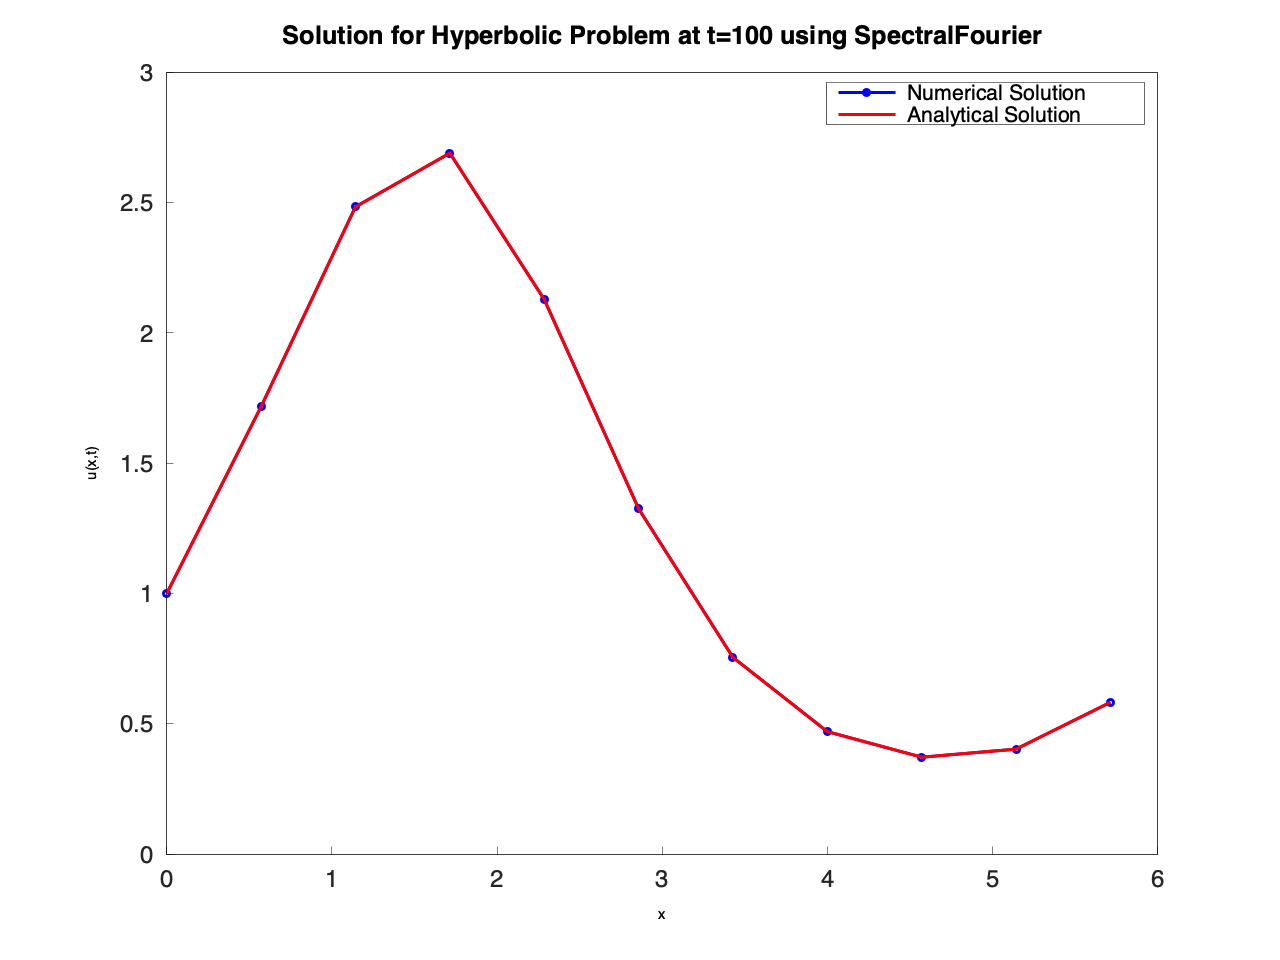
\includegraphics[width=\textwidth]{media/hyperbolic_SpectralFourier_100.png}
		\caption{Spectral Fourier at $t=100$}
		\label{sfig:sublabel4}
	\end{subfigure}\\
	\begin{subfigure}{0.5\textwidth}
		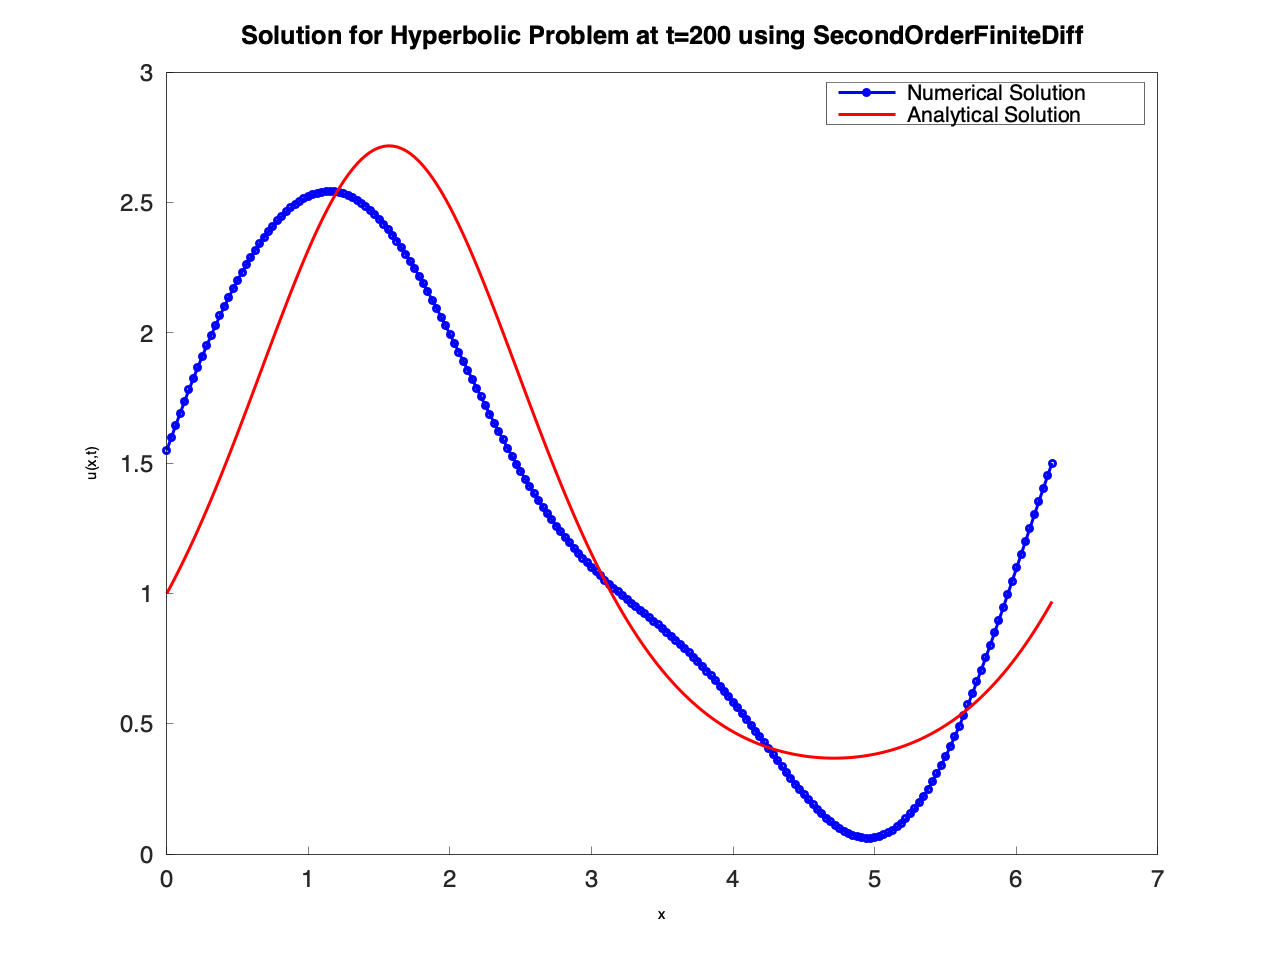
\includegraphics[width=\textwidth]{media/hyperbolic_SecondOrderFiniteDiff_200.png}
		\caption{Second Order at $t=200$}
		\label{sfig:sublabel5}
	\end{subfigure}%
	~
	\begin{subfigure}{0.5\textwidth}
		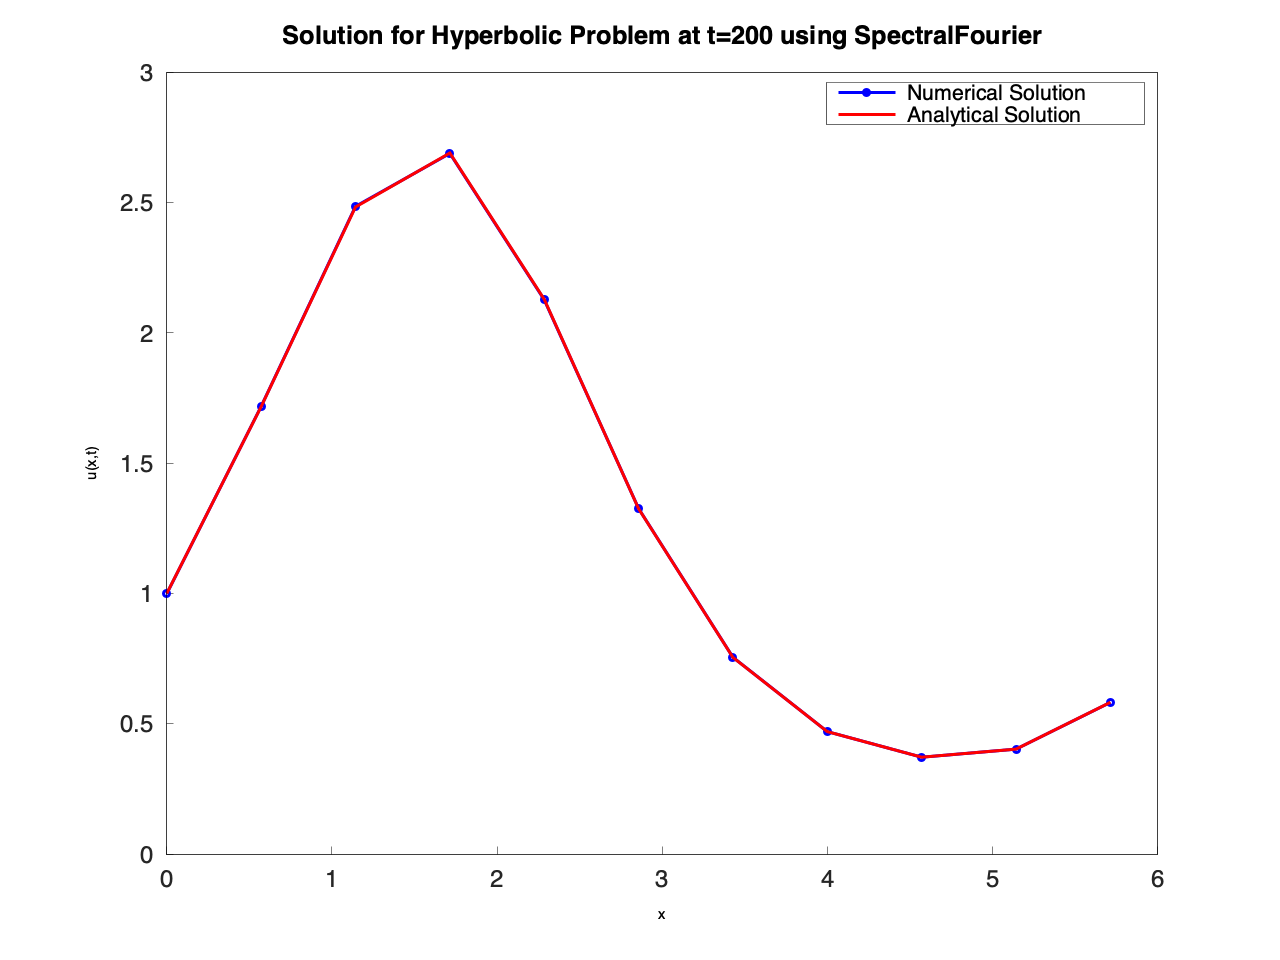
\includegraphics[width=\textwidth]{media/hyperbolic_SpectralFourier_200.png}
		\caption{Spectral Fourier at $t=200$}
		\label{sfig:sublabel6}
	\end{subfigure}

	\caption{\textbf{Comparison of Second Order Finite Difference and Spectral Fourier}
	}
	\label{fig:figureLabel}
\end{figure}


\end{document}
